\documentclass[fontsize=12]{article}

\pagestyle{empty}

\usepackage{amsmath}
\usepackage{amsfonts}
\usepackage{amssymb}
\usepackage{rotating}
\usepackage{enumerate}
\usepackage[normalem]{ulem}
\usepackage[dvipsnames]{xcolor} %allows use of color
%\usepackage{color}
%\usepackage{listings}
\usepackage{graphicx} %for adding pictures
\newcommand{\kB}{k_{\mathrm{B}}}
\newcommand{\kT}{\kB T}

\newcommand{\vek}[1]{\boldsymbol{#1}}          % vector symbol
\newcommand{\dif}{\mathrm{d}}                  % the d in integrals
\newcommand{\me}{\mathrm{e}}                   % Euler's e
\newcommand{\vekprod}{\! \cdot \!}
\newcommand{\eexp}[1]{\me^{\displaystyle #1}}
\newcommand{\eeexp}[1]{\me^{#1}}
\newcommand{\eeeexp}[1]{\exp \left( #1 \right)}
\newcommand{\mean}[1]{\left<#1\right>}
\newcommand{\abs}[1]{\left|#1\right|}
\newcommand{\orderof}[1]{\mathcal{O}\left(#1\right)}
\def\Real{\hbox{I\kern-.1667em\hbox{R}}}
\newcommand{\ffrac}[2]{\frac{\displaystyle #1}{\displaystyle #2}}
\newcommand{\ket}[1]{\left| #1 \right>}
\newcommand{\grad}{\vek{\nabla}}
\renewcommand{\Re}{\operatorname{Re}}
\renewcommand{\Im}{\operatorname{Im}}

\definecolor{MyGreen}{RGB}{27, 94, 20}
\newcommand*{\soln}[1]{\color{MyGreen}{{#1}}\color{black}}

\setlength{\oddsidemargin}{0.25cm}
\setlength{\textwidth}{6in}
\setlength{\topmargin}{0in}
\setlength{\headsep}{0in}
\setlength{\textheight}{8.9in}

\newcounter{problemcounter}  
\newenvironment{problemlist}
 {\begin{list}{\textbf{Problem \arabic{problemcounter}.}~}{\usecounter{problemcounter} \labelsep=0em \labelwidth=0em \leftmargin=0em \itemindent=0em}}
 {\end{list}}


\begin{document}
\begin{center}
\textbf{Homework Set 1} \\
Chemistry 553, Spring 2021 \\
Instructor: Lutz Maibaum \\
Student: Coire Gavin-Hanner \\
\vspace{1em}
\textbf{Due Friday, April 9th}
\end{center}

%\lstset{frame=shadowbox, rulesepcolor=\color{blue}}
%\lstinputlisting{/Users/lutz/c/python/ljmd/ljmd.py}

\begin{problemlist}

\item In this problem we will explore some basic concepts of random numbers.
\begin{enumerate}[(a)~]
\item Consider a random variable $\hat{X}$ that us uniformly distributed on the interval $[0,1]$, i.e., its probability distribution is
\begin{equation*}
p(x) = \begin{cases}
1 & \text{if } 0 \leq x \leq 1, \\
0 & \text{otherwise}.
\end{cases}
\end{equation*}
Calculate the mean and the variance of $\hat{X}$.\\
\soln{
	\begin{equation*}
	p(x) = P(\{x \in \Omega: \hat{X}(x) = x\}) = \begin{cases}
	1 & \text{if } 0 \leq x \leq 1, \\
	0 & \text{otherwise}.
	\end{cases}
\end{equation*}
This says that when $0 \leq x \leq 1$,  $\hat{X}(\omega) = \omega$, so we can solve for the mean and variance by the following:
\begin{align*}
	\text{mean} = \mean{\hat{X}} &= \int_\Omega \hat{X}(x)p(x)\,dx \\
	&= \int_o^1xp(x)\,dx = \left.\frac{x^2}{2}\right|_0^1 = \frac{1}{2}
\end{align*}
\begin{align*}
	\text{Variance} = var(\hat{X}) &= \mean{\hat{X}^2} - \mean{\hat{X}}^2\\
	&= \int_0^1 \hat{X}(x)^2p(x)\,dx - \mean{\hat{X}}^2\\
	&= \int_0^1 x^2p(x)\,dx - \mean{\hat{X}}^2\\
	&= \left.\frac{x^3}{3}\right|_0^1 - \frac{1}{4} = \frac{1}{12}
\end{align*}
}
\item Now consider two such random variable, $\hat{X}_1$ and $\hat{X}_2$, each distributed uniformly on $[0,1]$. Assume these random variables are independent. We can calculate the average of $\hat{X}_1$ and $\hat{X}_2$:
\begin{equation*}
\hat{S} = \ffrac{1}{2} \left( \hat{X}_1 +\hat{X}_2 \right),
\end{equation*}
which is itself a random variable. Calculate the probability distribution, the mean, and the variance of $\hat{S}$.\\
\soln{
	\begin{align*}
		\text{Probability distribution: ?}
	\end{align*}
	\begin{align*}
		\text{mean} = \mean{\hat{S}}	 &= \frac{1}{2}\left(\mean{\hat{X_1}}+\mean{\hat{X}_2}\right) = \frac{1}{2}\\
	\end{align*}
	\begin{align*}
		var(\hat{S}) &= \mean{\hat{S}^2} - \mean{\hat{S}}^2\\
		&= \mean{\left(\frac{1}{2}\left(\hat{X}_1 + \hat{X}_2\right)\right)^2} - \mean{\hat{S}}^2\\
		&= \frac{1}{4}\left(\mean{\hat{X}_1^2}+\mean{\hat{X}_2^2}+ 2\mean{\hat{X}_1}\mean{\hat{X}_2}\right)- \mean{\hat{S}}^2\\
		&= \frac{1}{24}
	\end{align*}
}
\item We can also take the average of $N$ independent, uniformly distributed random variables,
\begin{equation*}
\hat{S} = \ffrac{1}{N} \sum_{i=1}^N \hat{X}_i .
\end{equation*}
Based on what you found in part (a), what would you expect the probability distribution of $\hat{S}$ to be if $N$ is large? What about its expectation value and its variance?
\soln{
	If N is large, by the Central Limit Theorem, the probability density of $\hat{S}$ will be the Gaussian distribution that has parameters $\mu$ and $\sigma^2$ for the mean and variance, respectively. The mean will be equal to the mean of each individual $\hat{X}_i$ and the variance will be $\frac{1}{N}$ times the variance of each individual $\hat{X}_i$
}
\item Work through the posted ``Random Numbers'' Jupyter Notebook on random numbers. Do you find your expectations confirmed? Modify the last command block in that notebook to obtain the distribution of $\hat{S}$ for N=100. On the same plot, graph the Gaussian normal distribution with the mean and variance that you would expect for that value of $N$, and compare the two.\\
\soln{
Yes everything is what I expect. Please excuse the pixelated plot below. \\
}
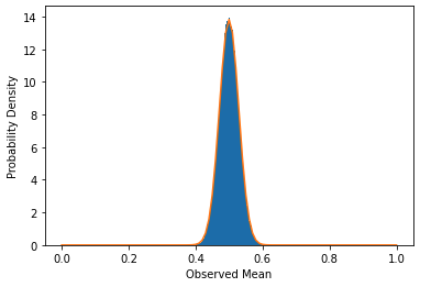
\includegraphics[scale=0.5]{gaussian}
\end{enumerate}

\item Consider a quantum-mechanical harmonic oscillator, which has states enumerated by a quantum number $n = 0, 1, 2, \dots$. As we will see later, the probability that the oscillator is in the $n$-th state is
\begin{equation*}
P(n) = \ffrac{1}{Z} \eexp{- \beta E_n}
\end{equation*}
where $\beta$ is a positive number, $E_n = \hbar \omega (n+1/2)$ is the energy of the $n$-th state, and $Z$ is a normalization constant. Find this normalization constant, i.e., find the expression of $Z$ such that
\begin{equation*}
\sum_{n=0}^\infty P(n) = 1 .
\end{equation*}
You can use the the following result for the \emph{geometric series}:
\begin{equation*}
\sum_{n=0}^\infty x^n = \ffrac{1}{1-x}
\end{equation*}
for all $\abs{x}<1$.
\soln{
	\begin{align*}
		\sum_{n=0}^\infty P(n) &= \sum_{n=0}^\infty  \ffrac{1}{Z} \eexp{- \beta \hbar \omega (n+1/2)} = 1\\
		&=\frac{1}{Z}\sum_{n=0}^\infty\eeexp{-\beta\hbar\omega n}\eeexp{-\frac{1}{2}\beta\hbar\omega} = 1\\
		&= \frac{\eeexp{-\frac{1}{2}\beta\hbar\omega}}{Z}\sum_{n=0}^\infty\left(\eeexp{-\beta\hbar\omega}\right)^n = 1 \\
		&= \frac{\eeexp{-\frac{1}{2}\beta\hbar\omega}}{Z}\frac{1}{1-\eeexp{\beta\hbar\omega}} = 1\\
		Z &= \frac{\eeexp{-\frac{1}{2}\beta\hbar\omega}}{1-\eeexp{\beta\hbar\omega}}
	\end{align*}
}
\item Show that the Gaussian normal distribution
\begin{equation*}
p(x) = \ffrac{1}{\sqrt{2\pi \sigma^2}} \eeexp{-\ffrac{(x-\mu)^2}{2 \sigma^2}} ,
\end{equation*}
where $\mu$ and $\sigma$ are two parameters, is normalized. In other words, show that
\begin{equation*}
\int_{-\infty}^\infty p(x) \dif x = 1 .
\end{equation*}
It might help to first show that
\begin{equation*}
  \ffrac{1}{\sqrt{2\pi}} \int_{-\infty}^\infty \eeexp{-\ffrac{x^2}{2}}  \dif x = 1 
\end{equation*}
by calculating
\begin{equation*}
\left( \int_{-\infty}^\infty \eeexp{-\ffrac{x^2}{2}}  \dif x  \right)^2 ,
\end{equation*}
which you can do by solving a two-dimensional integral in polar coordinates. 
\soln{
\begin{align*}
	\left( \int_{-\infty}^\infty \eeexp{-\ffrac{x^2}{2\sigma^2}}  \dif x  \right)^2 &= \int_{-\infty}^\infty e^{-\frac{x^2}{2\sigma^2}}\,dx\int_{-\infty}^\infty e^{-\frac{y^2}{2\sigma^2}}\,dy\\
	\text{we then use u-substitution to get $x'$ and $y'$:}\\
	&=2\sigma^2\int_{-\infty}^\infty \int_{-\infty}^\infty e^{-(x'^2 + y'^2)}\,dx'\,dy'\\
	&= 2\sigma^2\int_0^{2\pi}\int_0^\infty e^{-r^2}r\,dr\,d\Theta \\
	&= 4\pi\sigma^2\int_0^{\infty}re^{-r^2}\,dr \text{ we use u-substitution again} \\
	&= 2\pi\sigma^2\int_o^\infty e^s\,ds = 2\pi\sigma^2
\end{align*}
Now we can say that $\ffrac{1}{\sqrt{2\pi\sigma^2}} \int_{-\infty}^\infty \eeexp{-\ffrac{x^2}{2\sigma^2}}  \dif x = 1$ The only difference between this and the gaussian distribution is the $\mu$ term in the exponent of the gaussian. This does not change the integral. We are integrating over all real numbers so a translational shift in the position of the curve along the x-axis has no impact on the integral. Therefore, we can say that $\int_{-\infty}^\infty p(x) \dif x = 1$
}
\end{problemlist}  % enumeration of problems

%\begin{enumerate}[(a)~]
%\item
%\end{enumerate}
\end{document}
